% !TEX TS-program = pdflatexmk

\documentclass[14pt]{beamer}
\usepackage{newtxtext,newtxmath}
\usepackage{microtype}
\usepackage[english]{babel}
\usepackage{hyperref}
\usepackage{graphicx}
\usepackage{listings}
\lstloadlanguages{Python}
\lstset{language=Python}
\lstset{%
basicstyle=\ttfamily\bfseries,
keywordstyle=\color{blue}, emph={self}, emphstyle={\color{blue}},
identifierstyle=,
commentstyle=\color{brown},
stringstyle=\color{green!50!black},
showstringspaces=false,
emphstyle={[2]\color{purple}},
}
\usepackage{tikz}
\usepackage{pgfplots}
\usepackage{forest}
\usetikzlibrary{calc}
\usetikzlibrary{shapes}
\usetikzlibrary{positioning}
\usetikzlibrary{arrows}
\usepackage{array}
\newcolumntype{L}[1]{>{\raggedright\let\newline\\\arraybackslash\hspace{0pt}}m{#1}}

\mode<presentation>{
\usetheme{Madrid}
\definecolor{uabgreen}{cmyk}{.89,.31,.78,.17}
\usecolortheme[named=uabgreen]{structure}
\setbeamertemplate{navigation symbols}{}
\setbeamertemplate{footline}[frame number]
\setbeamertemplate{section in toc}[square]
\setbeamertemplate{subsection in toc}[square]
\setbeamertemplate{items}[square]
\setbeamercovered{transparent=5}
}

\newcommand{\keyword}[1]{{\color{blue}#1}}
\newcommand{\cmnt}[1]{{\color{gray}#1}}
\newcommand{\str}[1]{{\color{green!50!black}#1}}
\newcommand{\num}[1]{{\color{green!55!blue}#1}}
\newcommand{\defn}[1]{{\color{purple}#1}}

\newcommand{\limpl}{\Rightarrow}
\newcommand{\liff}{\Leftrightarrow}

\newcommand{\tab}{\hspace{1em}}

\author[Dr. Bethard]{Dr. Steven Bethard}
\institute[UAB CIS]{%
Computer and Information Sciences\\
University of Alabama at Birmingham}

\AtBeginSection[]
{
  \begin{frame}<beamer>{Outline}
    \tableofcontents[currentsection]
  \end{frame}
}

\tikzset{
  invisible/.style={opacity=0,text opacity=0},
  text visible on/.code={%
    \alt<#1>{}{\pgfkeysalso{text opacity=0}}
  },
  visible on/.code={%
    \alt<#1>{}{\pgfkeysalso{invisible}}
  },
  filled on/.code={%
    \alt<#1>{\pgfkeysalso{fill=gray}}{}
  },
  alt/.code n args={3}{%
    \alt<#1>{\pgfkeysalso{#2}}{\pgfkeysalso{#3}}
  },
}
\forestset{
  edge weight/.style={
    edge label={node[midway,above,sloped]{#1}}},
  invisible/.style={
    /tikz/invisible,
    edge={/tikz/invisible}},
  visible on filled on/.code n args={2}{%
    \alt<#1>{\alt<#2>{\pgfkeysalso{fill=gray}}{}}{\pgfkeysalso{invisible}}
  },
  visible on/.code={%
    \alt<#1>{}{\pgfkeysalso{invisible}}
  },
}

\newlength{\wumpusgridsize}
\newenvironment{wumpusgrid}[2]{%
\setlength{\wumpusgridsize}{#2}
\begin{tikzpicture}
\draw[very thick,step=\wumpusgridsize] (0,0) grid (#1\wumpusgridsize, #1\wumpusgridsize);
}{%
\end{tikzpicture}
}
\newcommand{\wumpustop}[5][]{%
\only<#2>{\node[#1] at (#3\wumpusgridsize+0.5\wumpusgridsize,#4\wumpusgridsize+0.75\wumpusgridsize) {#5};}
}
\newcommand{\wumpusbottom}[5][]{%
\only<#2>{\node[#1] at (#3\wumpusgridsize+0.5\wumpusgridsize,#4\wumpusgridsize+0.25\wumpusgridsize) {#5};}
}
\newcommand{\wumpusagent}[3]{\wumpusbottom{#1}{#2}{#3}{\fbox{A}}}
\newcommand{\wumpuspercept}[4]{%
\only<#1>{\node[red,inner sep=0pt] at (#2\wumpusgridsize+0.25\wumpusgridsize,#3\wumpusgridsize+0.75\wumpusgridsize) {\textbf{#4}};}
}
\newcommand{\wumpusknowledge}[4]{%
\only<#1>{\node[draw,cloud,inner sep=0pt,text width=1em,align=center] at (#2\wumpusgridsize+0.75\wumpusgridsize,#3\wumpusgridsize+0.75\wumpusgridsize) {\footnotesize #4};}
}

\lstset{emph={[2]__init__,__str__}}

\title{Adversarial Search}
\date[]{28 Jan 2016}

\newcommand{\tictactoe}[9]{
\begin{tabular}{@{} c @{\hspace{0.2em}} | @{\hspace{0.2em}} c @{\hspace{0.2em}} | @{\hspace{0.2em}} c @{\hspace{0.2em}}}
#1 & #2 & #3 \\
\hline
#4 & #5 & #6 \\
\hline
#7 & #8 & #9 \\
\end{tabular}
}
\newcommand{\abcutil}[3]{(#1,#2,#3)}
\newcommand{\utilab}[3]{%
#1{\tiny
\begin{tabular}{ l @{} >{\centering\arraybackslash}m{2.2em} @{}}
$\geq$ & $#2$ \\
$\leq$ & $#3$
\end{tabular}}}

\begin{document}

\begin{frame}
  \titlepage
\end{frame}

\begin{frame}{Outline}
  \tableofcontents
\end{frame}

\section{Describing Games}
\subsection{Games as Search}
\begin{frame}{Games as Search}
	\begin{block}{Games as Search}
		\begin{description}
			\item[Initial] A board position and which player is to move
			\item[Actions] Moves and resulting states
			\item[Goal] A terminal state, where the game has ended
			\item[Score] Based on utility function, e.g. +1 win, -1 lose
		\end{description}
	\end{block}
	\pause
	\begin{block}{Game Types}
		\centering
		\hyphenpenalty=10000
		\begin{tabular}{ L{0.2\textwidth} | L{0.3\textwidth} | L{0.3\textwidth}}
			                    & Deterministic               & Stochastic \\
			\hline
			Perfect information       & \uncover<3->{chess, checkers, go, reversi}     & \uncover<4->{backgammon, monopoly} \\
			\hline
			Imperfect information    & \uncover<5->{battleship, blind tic-tac-toe}          & \uncover<6->{bridge, poker, scrabble} \\
		\end{tabular}
	\end{block}
\end{frame}
\subsection{Game Search Trees}
\begin{frame}{Tic-Tac-Toe Game Tree}
	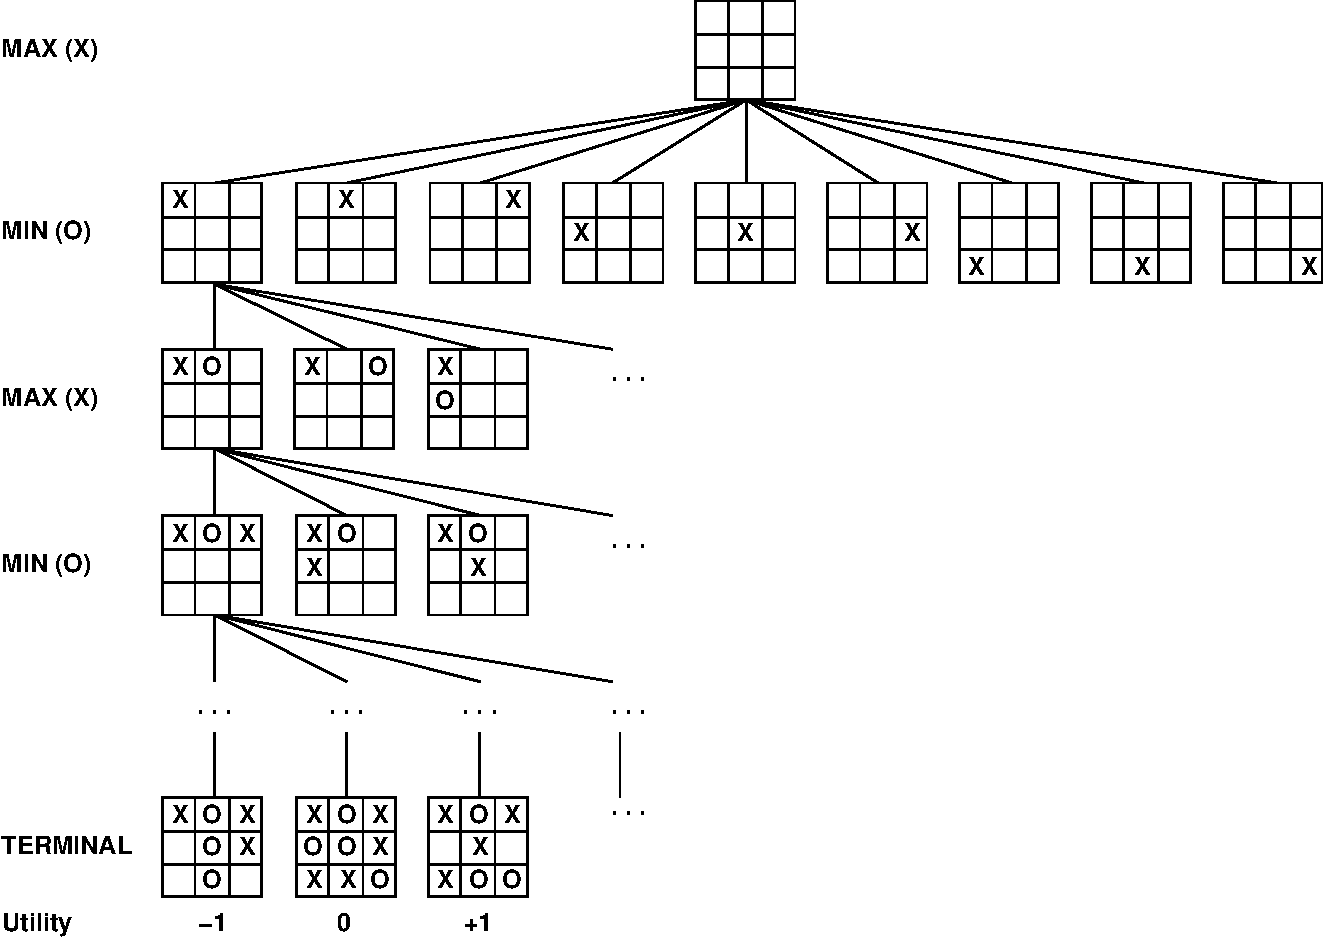
\includegraphics[width=4in]{tictactoe.pdf}
\end{frame}

\section{Deterministic Games}
\subsection{Minimax}
\begin{frame}[fragile,label=minimax-example]{Minimax}
\begin{block}{Idea}
\begin{itemize}
\item Expect other player to minimize your utility
\item Choose action that maximizes the minimized utility
\end{itemize}
\end{block}
\begin{center}
\small
\begin{forest}
left action/.style={
  edge label={node[midway,left]{\small #1}}},
middle action/.style={
  edge label={node[midway,left=-0.25em]{\small #1}}},
right action/.style={
  edge label={node[midway,right]{\small #1}}},
for tree={minimum size=1.5em,l sep=3em,s sep=1em}
[{},phantom
  [{Max Player},edge=invisible
    [{Min Player},edge=invisible
      [{Max Player},invisible]
    ]
  ]
  [{3},edge=invisible,for tree={draw},text visible on={11}
    [{3},left action={$a_1$},visible on={2-10},text visible on={4-10}
      [{3},left action={$b_1$},visible on={3}]
      [{12},middle action={$b_2$},visible on={3}]
      [{8},right action={$b_3$},visible on={3}]
    ]
    [{2},middle action={$a_2$},visible on={5-10},text visible on={7-10}
      [{2},left action={$c_1$},visible on={6}] 
      [{4},middle action={$c_2$},visible on={6}]
      [{6},right action={$c_3$},visible on={6}]
    ]
    [{2},right action={$a_3$},visible on={8-10},text visible on={10-10}
      [{14},left action={$d_1$},visible on={9}]
      [{5},middle action={$d_2$},visible on={9}]
      [{2},right action={$d_3$},visible on={9}]
    ]
  ]
]
\end{forest}
\end{center}
\end{frame}
\begin{frame}{Minimax Exercise}
	\begin{columns}
		\begin{column}{2in}
			\begin{block}{Build Minimax Tree}
				\begin{itemize}
					\item It is X's turn
					\item Scoring: \\
						\begin{tabular}{lr}
							X Wins      & +1 \\
							X Loses     & -1 \\
							X and O Tie &  0 \\
						\end{tabular}
				\end{itemize}
			\end{block}
		\end{column}
		\begin{column}{2in}
			\centering
			\Huge
			\tictactoe{O}{X}{X}{X}{ }{ }{O}{O}{ }
		\end{column}
	\end{columns}
\end{frame}
\begin{frame}{Minimax Exercise}
\begin{center}
\scriptsize
\begin{forest}
for tree={align=center,s sep=2em}
[{\tictactoe{O}{X}{X}{X}{ }{ }{O}{O}{ } \\ $f(n) = 0$}
  [{\tictactoe{O}{X}{X}{X}{X}{ }{O}{O}{ } \\ $f(n) = -1$}
    [{\tictactoe{O}{X}{X}{X}{X}{O}{O}{O}{ } \\ $f(n) = 0$}
      [{\tictactoe{O}{X}{X}{X}{X}{O}{O}{O}{X} \\ $f(n) = 0$}]
    ]
    [{\tictactoe{O}{X}{X}{X}{X}{ }{O}{O}{O} \\ $f(n) = -1$}]
  ]
  [{\tictactoe{O}{X}{X}{X}{ }{X}{O}{O}{ } \\ $f(n) = -1$}
    [{\tictactoe{O}{X}{X}{X}{O}{X}{O}{O}{ } \\ $f(n) = +1$}
      [{\tictactoe{O}{X}{X}{X}{O}{X}{O}{O}{X} \\ $f(n) = +1$}]
    ]
    [{\tictactoe{O}{X}{X}{X}{ }{X}{O}{O}{O} \\ $f(n) = -1$}]
  ]
  [{\tictactoe{O}{X}{X}{X}{ }{ }{O}{O}{X} \\ $f(n) = 0$}
    [{\tictactoe{O}{X}{X}{X}{O}{ }{O}{O}{X} \\ $f(n) = +1$}
      [{\tictactoe{O}{X}{X}{X}{O}{X}{O}{O}{X} \\ $f(n) = +1$}]
    ]
    [{\tictactoe{O}{X}{X}{X}{ }{O}{O}{O}{X} \\ $f(n) = 0$}
      [{\tictactoe{O}{X}{X}{X}{X}{O}{O}{O}{X} \\ $f(n) = 0$}]
    ]
  ]
]
\end{forest}
\end{center}
\end{frame}
\begin{frame}[fragile,label=minimax-properties]{Minimax Properties}
\begin{center}
\small
\begin{forest}
left action/.style={
  edge label={node[midway,left]{\small #1}}},
middle action/.style={
  edge label={node[midway,left=-0.25em]{\small #1}}},
right action/.style={
  edge label={node[midway,right]{\small #1}}},
for tree={minimum size=1.5em,l sep=3em,s sep=1.2em}
[{},phantom
  [{Max Player},edge=invisible
    [{Min Player},edge=invisible
      [{Max Player},invisible]
    ]
  ]
  [{3},edge=invisible,for tree={draw},text opacity=0
    [{3},left action={$a_1$},for children=invisible
      [{3},left action={$b_1$}]
      [{12},middle action={$b_2$}]
      [{8},right action={$b_3$}]
    ]
    [{2},middle action={$a_2$},text opacity=0
      [{2},left action={$c_1$}] 
      [{4},middle action={$c_2$}]
      [{6},right action={$c_3$}]
    ]
    [{2},right action={$a_3$},text opacity=0,for children=invisible
      [{14},left action={$d_1$}]
      [{5},middle action={$d_2$}]
      [{2},right action={$d_3$}]
    ]
  ]
]
\end{forest}
\end{center}
\begin{tabular}{ll}
Complete? & \uncover<2->{Yes, if tree is finite} \\
Optimal?   & \uncover<3->{Yes, for optimal opponent} \\
Time? & \uncover<4->{$O(b^m)$, all nodes in the tree} \\
Space? & \uncover<5->{$O(bm)$, like depth first search} \\
\end{tabular}
\end{frame}
\begin{frame}{Multiplayer Minimax}
\begin{center}
\scriptsize
\begin{forest}
for tree={align=center,minimum size=1.5em,l sep=3em,s sep=1.25em}
[{},phantom
  [{Player 0},edge=invisible
    [{Player 1},edge=invisible
      [{Player 2},edge=invisible
        [{Player 0},edge=invisible]
      ]
    ]
  ]
  [{\abcutil{1}{2}{6}},for tree={draw},text visible on={8-}
    [{\abcutil{1}{2}{6}},text visible on={4-}
      [{\abcutil{1}{2}{6}},text visible on={2-}
        [{\abcutil{1}{2}{6}}
          [{\ldots},draw=none]
        ]
        [{\abcutil{4}{2}{3}}
          [{\ldots},draw=none]
        ]
      ]
      [{\abcutil{6}{1}{2}},text visible on={3-}
        [{\abcutil{6}{1}{2}}
          [{\ldots},draw=none]
        ]
        [{\abcutil{7}{4}{1}}
          [{\ldots},draw=none]
        ]
      ]
    ]
    [{\abcutil{1}{5}{2}},text visible on={7-}
      [{\abcutil{1}{5}{2}},text visible on={5-}
        [{\abcutil{5}{1}{1}}
          [{\ldots},draw=none]
        ]
        [{\abcutil{1}{5}{2}}
          [{\ldots},draw=none]
        ]
      ]
      [{\abcutil{5}{4}{5}},text visible on={6-}
        [{\abcutil{7}{7}{1}}
          [{\ldots},draw=none]
        ]
        [{\abcutil{5}{4}{5}}
          [{\ldots},draw=none]
        ]
      ]
    ]
  ]
]
\end{forest}
\end{center}
\end{frame}

\begin{frame}{Alpha-Beta Pruning}
	\begin{columns}
		\begin{column}{2in}
			\begin{block}{Idea}
				If $m$ is a better choice, then $n$ will never be reached
			\end{block}
			\begin{block}<2->{Alpha-Beta Bookkeeping}
				\begin{itemize}
					\item[$\alpha$] Best value for Player \\ (the highest value)
					\item[$\beta$] Best value for Opp \\ (the lowest value)
				\end{itemize}
			\end{block}
		\end{column}
		\begin{column}{2in}
			\begin{center}
				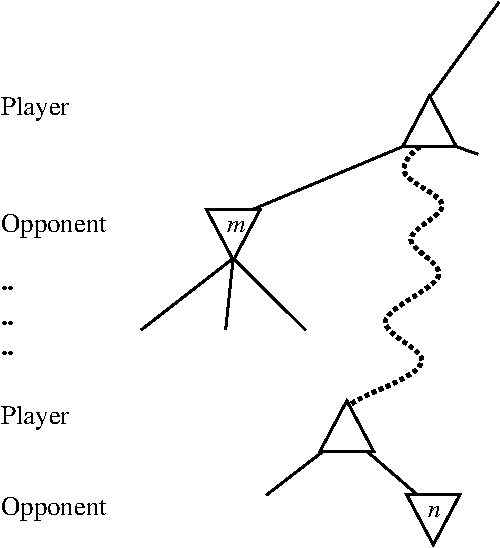
\includegraphics[width=2in]{alpha-beta-general.pdf}
			\end{center}
		\end{column}
	\end{columns}
\end{frame}
\subsection{Alpha-Beta Pruning Example}
\begin{frame}[label=alpha-beta-pruning-example]{Alpha-Beta Pruning}
% from http://www.cs.ucla.edu/~rosen/161/notes/alphabeta.html
\begin{center}
\footnotesize
\begin{forest}
pruned/.style={draw=none,content={---}}
[{},phantom,for tree={align=center}
  [{Max},for tree={edge=invisible,l sep*=1.25}
    [{Min}
      [{Max}
	[{Min}
	  [{Max},invisible]
	]
      ]
    ]
  ]
  [{\utilab{\visible<41->{3}}{\alt<25->{3}{-\infty}}{+\infty}},for tree={draw}
    [{\utilab{\visible<24->{3}}{-\infty}{\alt<16->{3}{+\infty}}},visible on={2-40}
      [{\utilab{\visible<15->{3}}{\alt<9->{3}{-\infty}}{+\infty}},visible on={3-23}
        [{\utilab{\visible<8->{3}}{-\infty}{\alt<6->{3}{+\infty}}},visible on={4-14}
          [{3},visible on={5-7}]
          [{17},visible on={7}]
        ]
        [{\utilab{\visible<14->{2}}{3}{\alt<12->{2}{+\infty}}},visible on={10-14}
          [{2},visible on={11-13}]
          [{12},pruned,visible on={13}]
        ]
      ]
      [{\utilab{\visible<23->{15}}{\alt<21->{15}{-\infty}}{3}},visible on={17-23}
        [{\utilab{\visible<20->{15}}{-\infty}{3}},visible on={18-22}
          [{15},visible on={19}]
        ]
        [{},pruned,visible on={22}
          [{25},invisible]
          [{0},invisible]
        ]
      ]
    ]
    [{\utilab{\visible<40->{3}}{3}{\alt<38->{3}{+\infty}}},visible on={26-40}
      [{\utilab{\visible<37->{3}}{3}{+\infty}},visible on={27-39}
        [{\utilab{\visible<32->{2}}{3}{\alt<30->{2}{+\infty}}}, visible on={28-36}
          [{2},visible on={29-31}]
          [{5},pruned,visible on={31}]
        ]
        [{\utilab{\visible<36->{3}}{3}{\alt<35->{3}{+\infty}}},visible on={33-36}
          [{3},visible on={34-35}]
        ]
      ]
      [{},pruned,visible on={39}
        [{},invisible
          [{2},invisible]
          [{14},invisible]
        ]
      ]
    ]
  ]
]
\end{forest}
\end{center}
\end{frame}
\begin{frame}[label=alpha-beta-pruning-properties]{Alpha-Beta Pruning Properties}
\begin{center}
\footnotesize
\begin{forest}
pruned/.style={draw=none,content={---}}
[{},phantom,for tree={align=center}
  [{Max},for tree={edge=invisible,l sep*=1.25}
    [{Min}
      [{Max}
	[{Min}]
      ]
    ]
  ]
  [{\utilab{\invisible{3}}{-\infty}{+\infty}},for tree={draw}
    [{\utilab{\invisible{3}}{-\infty}{3}}
      [{\utilab{3}{3}{+\infty}}
        [{\utilab{3}{-\infty}{3}},invisible]
        [{\utilab{2}{3}{2}},invisible]
      ]
      [{\utilab{\invisible{15}}{15}{3}}
        [{\utilab{15}{-\infty}{3}}]
        [{},pruned]
      ]
    ]
    [{\utilab{3}{3}{+\infty}},invisible
      [{\utilab{3}{3}{+\infty}},invisible]
      [{},pruned,invisible]
    ]
  ]
]
\end{forest}
\end{center}
	\begin{block}{Time Complexity}
		\begin{itemize}
			\pause
			\item ``Perfectly'' ordered branches gives $O(b^{m/2})$
			\pause
			\item Still exponential, but doubles solvable depth
		\end{itemize}
	\end{block}
\end{frame}

\subsection{Approximate Solutions}
\begin{frame}[fragile]{Approximate Solutions}
	\begin{block}{Problem}
		Even with Alpha-Beta Pruning, chess space is still $35^{50}$
	\end{block}
	\pause
	\begin{block}{Solution}
		Don't search the entire tree:
		\begin{semiverbatim}\scriptsize\bfseries
		    \keyword{if} problem.\alt<3->{\alert{is_past_cutoff}}{is_terminal}(state):
		        \keyword{return} problem.\alt<3->{\alert{get_estimated_utility}}{get_utility}(state)
		
		\end{semiverbatim}
	\end{block}
	\pause\pause
	\begin{block}{Example}
		\begin{itemize}
			\item Given 100 seconds
			\item Given ability to explore $10^4$ nodes/second
			\item Can explore to depth $\approx 8$ ($10^6 \approx 35^{8/2}$)
		\end{itemize}
	\end{block}
\end{frame}
\begin{frame}{Evaluation Functions}
	\begin{block}{Necessary Properties}
		\begin{itemize}
			\item Quickly computable
			\item For terminals, $\textsc{Eval}(s)$ orders by utility
			\item For nonterminals, $\textsc{Eval}(s)$ correlates with winning
		\end{itemize}
	\end{block}
	\pause
	\begin{block}{Typical Approach}
		Weighted linear combination of features:
		\[\mbox{\sc Eval}(s) = w_1 f_1(s) + w_1 f_2(s) + \ldots + w_n f_n(s)\]
	\end{block}
\end{frame}
\begin{frame}{Example Evaluation Function}
	\centering
	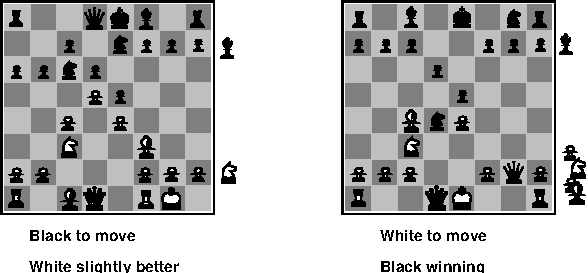
\includegraphics[height=1.75in]{chess-evaluation.pdf}
	\begin{block}{Weighted Features}
		\small
		$
		\begin{array}{rcl}
			w_{\mbox{\scriptsize pawn}}  \cdot f_{\mbox{\scriptsize pawn}}(s)  & = & 1 \cdot (\mbox{white pawns} - \mbox{black pawns})   \\
			\ldots                                                             & = & \ldots \\
			w_{\mbox{\scriptsize queen}} \cdot f_{\mbox{\scriptsize queen}}(s) & = & 9 \cdot (\mbox{white queens} - \mbox{black queens})
		\end{array}
		$
	\end{block}
\end{frame}
\begin{frame}[label=evaluation-function-exercise]{Design an Evaluation Function}
\begin{block}{Extended Tic-Tac-Toe}
\begin{itemize}
\item $N \times N$ board
\item $K$ in a row wins
\end{itemize}
\end{block}
\bigskip
Must satisfy:
\begin{itemize}
\item Quickly computable
\item 
$\begin{array}[t]{lll}
\lefteqn{\forall x,t,o \! \in \! \textsc{Terminals},}\\
& \lefteqn{\textsc{Util}(x) = +1 \wedge \textsc{Util}(t) = 0 \wedge \textsc{Util}(o) = -1} \\
& & \implies  \textsc{Eval}(x) > \textsc{Eval}(t) > \textsc{Eval(o)}
\end{array}$ 
\item
$\forall s \! \in \! \textsc{Nonterminals}, \textsc{Eval}(s)$ correlates with chance of +1
\end{itemize}
\end{frame}
\begin{frame}{Deterministic Games in Practice}
	Checkers:
		% http://webdocs.cs.ualberta.ca/~chinook/
		\begin{itemize}
			\item\small 1995: Chinook ``Man-Machine World Champion'' (1-0-31)
			\item\small 2007: Chinook's creators ``proved'' it cannot lose
			\item\small End-game database for all $\leq 8$ piece states
		\end{itemize}
	Chess:
		\begin{itemize}
			\item\small 1997: Deep Blue defeated Garry Kasparov (2-1-3)
			\item\small Searches 6-40 plies; end-game database for $\leq 5$ piece states
			\item\small 2002,'04,'06,'09,'11,'13: Junior wins World Computer Chess
		\end{itemize}
	Go:
		\begin{itemize}
			\item\small Branching factor starts at 361 $\Rightarrow$ Monte Carlo methods
			\item\small 2015: Computers still rank as advanced amateurs
			\item\small 2016: AlphaGo beats professional player Fan Hui, 5-0 %http://googleresearch.blogspot.com/2016/01/alphago-mastering-ancient-game-of-go.html
		\end{itemize}
\end{frame}

\section{Nondeterministic Games}

\subsection{Describing Nondeterministic Games}
\begin{frame}{Nondeterministic Game: Backgammon}
	\begin{center}
		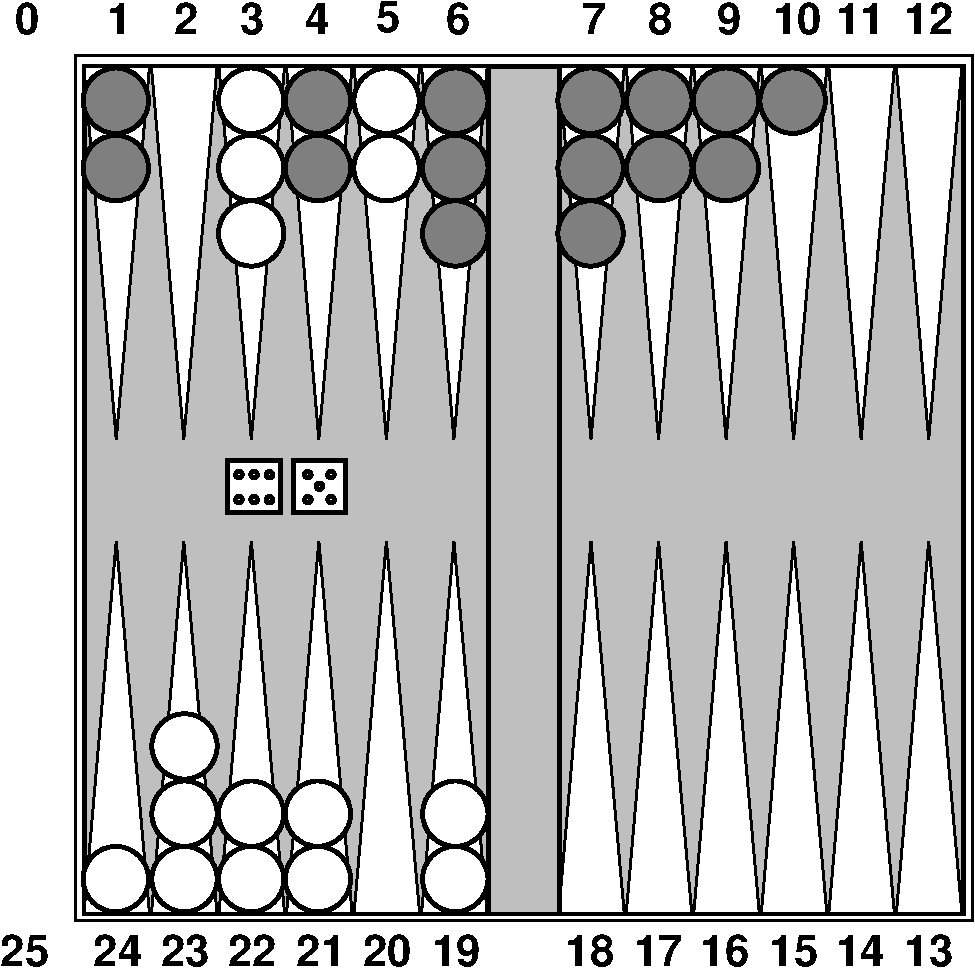
\includegraphics[height=2.5in]{backgammon-position.pdf}
	\end{center}
\end{frame}
\begin{frame}{Backgammon Game Tree}
	\begin{center}
		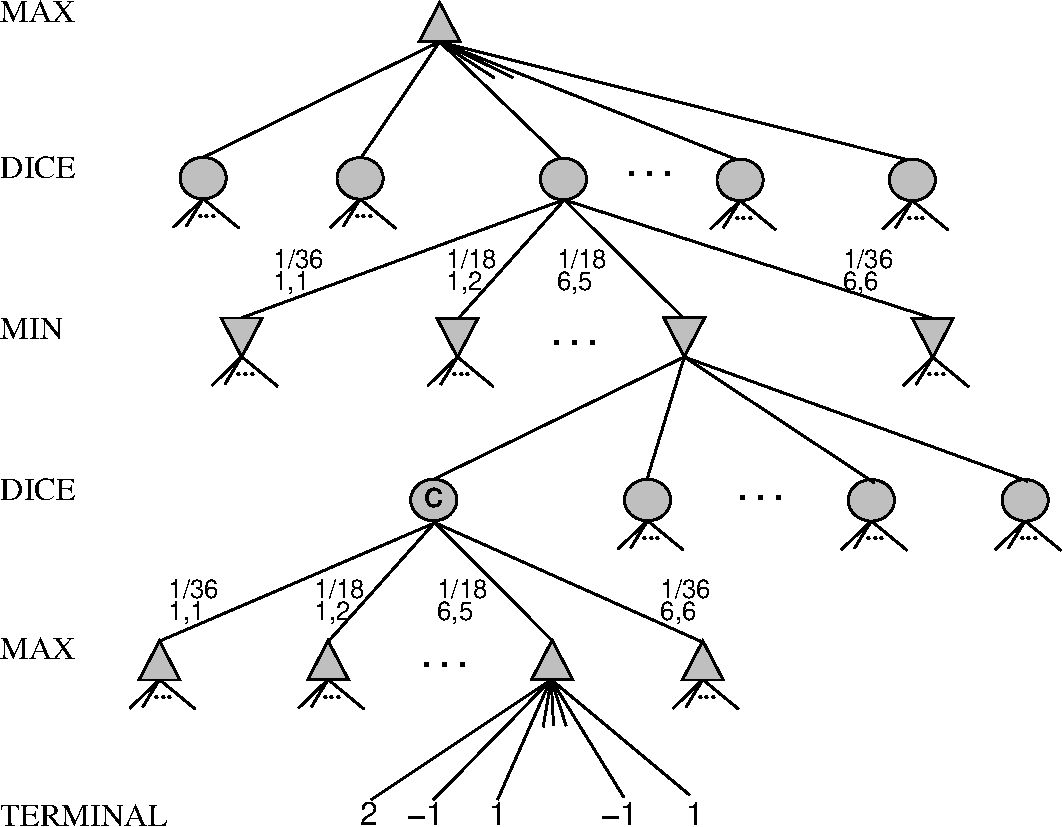
\includegraphics[height=2.5in]{backgammon-tree.pdf}
	\end{center}
\end{frame}

\subsection{Expectiminimax}
\begin{frame}[label=expectiminimax]{Expectiminimax}
\begin{block}{\centering Expected Values for Chance Nodes}
\[f(n) = \sum\limits_{s \in \textsc{\scriptsize Successors}(n)}{P(s) \cdot f(s)}\]
\end{block}
\begin{center}
\small
\begin{forest}
pruned/.style={draw=none,content={---}}
[{},phantom,for tree={align=center,l sep*=1.1}
  [{Max},for tree={edge=invisible}
    [{Chance}
      [{Min}
	[{Util},invisible]
      ]
    ]
  ]
  [{3},for tree={draw},text visible on={15-}
    [{3},visible on={2-14},text visible on={8-}
      [{2},edge weight={0.5},visible on={3-7},text visible on={5-}
        [{2},visible on={4}]
        [{4},visible on={4}]
      ]
      [{4},edge weight={0.5},visible on={3-7},text visible on={7-}
        [{7},visible on={6}]
        [{4},visible on={6}]
      ]
    ]
    [{-1},visible on={2-14},text visible on={14-}
      [{0},edge weight={0.5},visible on={9-13},text visible on={11-}
        [{6},visible on={10}]
        [{0},visible on={10}]
      ]
      [{-2},edge weight={0.5},visible on={9-13},text visible on={13-}
        [{5},visible on={12}]
        [{-2},visible on={12}]
      ]
    ]
  ]
]
\end{forest}
\end{center}
\end{frame}
\begin{frame}{Expectiminimax Practice}
	\begin{block}{A Simple Game}
		\begin{itemize}
			\item Deck contains J, Q, K, K in a random order
			\item A card is drawn and Player 1 either:
				\begin{itemize}
					\item Ends the game, or
					\item Another card is drawn and Player 2 either:
						\begin{itemize}
							\item Ends the game, or
							\item Another card is drawn and the game ends
						\end{itemize}
				\end{itemize}
			\item Utility is determined by the last card drawn
			\item J scores -1, Q scores 0, and K scores +1
		\end{itemize}
	\end{block}
\end{frame}
\begin{frame}[label=expectiminimax-practice]{Expectiminimax Practice}
\begin{center}
\tiny
\begin{forest}
[{},phantom,for tree={align=center,l sep=3em}
  [{Chc},for tree={edge=invisible}
    [{Max}
      [{Chc}
        [{Min}
          [{Chc}]
        ]
      ]
    ]
  ]
  [{+$\frac{7}{12}$},for tree={draw,s sep=1.35em}
    [{+$\frac{1}{3}$},edge weight={J$\frac{1}{4}$}
      [{-1},edge weight={\textsc{Keep}}]
      [{+$\frac{1}{3}$},edge weight={\textsc{Draw}}
        [{0},edge weight={Q$\frac{1}{3}$}
          [{0},edge weight={\textsc{Keep}}]
          [{+1},edge weight={\textsc{Draw}}
            [{+1},edge weight={K$\frac{2}{2}$}]
          ]
        ]
        [{$+\frac{1}{2}$},edge weight={K$\frac{2}{3}$}
          [{+1},edge weight={\textsc{Keep}}]
          [{$+\frac{1}{2}$},edge weight={\textsc{Draw}}
            [{0},edge weight={Q$\frac{1}{2}$}]
            [{+1},edge weight={K$\frac{1}{2}$}]
          ]
        ]
      ]
    ]
    [{0},edge weight={Q$\frac{1}{4}$}
      [{0},edge weight={\textsc{Keep}}]
      [{-$\frac{1}{3}$},edge weight={\textsc{Draw}}
        [{-1},edge weight={J$\frac{1}{3}$}
          [{-1},edge weight={\textsc{Keep}}]
          [{+1},edge weight={\textsc{Draw}}
            [{+1},edge weight={K$\frac{2}{2}$}]
          ]
        ]
        [{0},edge weight={K$\frac{2}{3}$}
          [{+1},edge weight={\textsc{Keep}}]
          [{0},edge weight={\textsc{Draw}}
            [{-1},edge weight={J$\frac{1}{2}$}]
            [{+1},edge weight={K$\frac{1}{2}$}]
          ]
        ]
      ]
    ]
    [{+1},edge weight={K$\frac{2}{4}$}
      [{+1},edge weight={\textsc{Keep}}]
      [{-$\frac{1}{2}$},edge weight={\textsc{Draw}}
        [{-1},edge weight={J$\frac{1}{3}$}
          [{-1},edge weight={\textsc{Keep}}]
          [{+$\frac{1}{2}$},edge weight={\textsc{Draw}}
            [{0},edge weight={Q$\frac{1}{2}$}]
            [{+1},edge weight={K$\frac{1}{2}$}]
          ]
        ]
        [{0},edge weight={Q$\frac{1}{3}$}
          [{0},edge weight={\textsc{Keep}}]
          [{0},edge weight={\textsc{Draw}}
            [{-1},edge weight={J$\frac{1}{2}$}]
            [{+1},edge weight={K$\frac{1}{2}$}]
          ]
        ]
        [{-$\frac{1}{2}$},edge weight={K$\frac{1}{3}$}
          [{+1},edge weight={\textsc{Keep}}]
          [{-$\frac{1}{2}$},edge weight={\textsc{Draw}}
            [{-1},edge weight={J$\frac{1}{2}$}]
            [{0},edge weight={Q$\frac{1}{2}$}]
          ]
        ]
      ]
    ]
  ]
]
\end{forest}
\end{center}
\end{frame}
\begin{frame}[label=using-expectiminimax]{Using Expectiminimax}
	\begin{block}{Expectiminimax Properties}
		\begin{tabular}{@{} ll @{}}
			Complete? & \uncover<2->{Yes, if tree is finite (both moves and ``rolls'')} \\
			Optimal? & \uncover<3->{Yes} \\
			Time? & \uncover<4->{$O(b^mn^m)$, all nodes, all ``roll'' sequences} \\
		\end{tabular}
	\end{block}
	\begin{block}{Consequences}<5->
		\begin{tabular}{@{} ll @{}}
			Node Likelihood? & \uncover<6->{Decreases with depth} \\
			Alpha-Beta Pruning? & \uncover<7->{Effectiveness decreased} \\
		\end{tabular}
	\end{block}
	\begin{block}{Real-World Example: TD-Gammon}<8->
		\begin{itemize}
			\item Depth 2-3 search, no Alpha-Beta pruning
			\item Neural network eval function trained by self-play
		\end{itemize}
	\end{block}
\end{frame}
\begin{frame}[label=expectiminimax-utility]{Utilities: Minimax vs. Expectiminimax}

{\scriptsize
\begin{forest}
utility/.style={draw=none}
[{},phantom,for tree={align=center},s sep=8em
  [{Max},for tree={edge=invisible}
    [{Min}
      [{Util},invisible]
    ]
  ]
  [{2},for tree={draw,s sep=1.5em}
    [{2}
      [{2},utility]
      [{3},utility]
    ]
    [{1}
      [{1},utility]
      [{4},utility]
    ]
  ]
  [{20},for tree={draw}
    [{20}
      [{20},utility]
      [{30},utility]
    ]
    [{1}
      [{1},utility]
      [{400},utility]
    ]
  ]
]
\end{forest}
}
\\\bigskip\bigskip
{\scriptsize
\visible<2->{
\begin{forest}
utility/.style={draw=none}
[{},phantom,for tree={align=center},s sep=1em
  [{Max},for tree={edge=invisible}
    [{Chc}
      [{Min}
        [{Util},invisible]
      ]
    ]
  ]
  [{2.1},for tree={draw,s sep=1.5em}
    [{2.1}
      [{2},edge weight={0.9}
        [{2},utility]
        [{2},utility]
      ]
      [{3},edge weight={0.1}
        [{3},utility]
        [{3},utility]
      ]
    ]
    [{1.3}
      [{1},edge weight={0.9}
        [{1},utility]
        [{1},utility]
      ]
      [{4},edge weight={0.1}
        [{4},utility]
        [{4},utility]
      ]
    ]
  ]
  [{40.9},for tree={draw}
    [{21}
      [{20},edge weight={0.9}
        [{20},utility]
        [{20},utility]
      ]
      [{30},edge weight={0.1}
        [{30},utility]
        [{30},utility]
      ]
    ]
    [{40.9}
      [{1},edge weight={0.9}
        [{1},utility]
        [{1},utility]
      ]
      [{400},edge weight={0.1}
        [{400},utility]
        [{400},utility]
      ]
    ]
  ]
]
\end{forest}
}
}
\\
\visible<3->{Evaluation function must be linear transform of true utility}
\end{frame}

\subsection{Partially Observable Games}
\begin{frame}[label=partially-observable-games]{Partially Observable Games}
Missing knowledge on opponent state
\begin{itemize}
\item Poker, Blackjack, Bridge, etc.
\item<2-> Just average over all possible unknowns? \visible<9->{\alert<9->{No!}}
\end{itemize}
\bigskip
\uncover<3->{Problems with \emph{averaging over clairvoyance}}
\begin{itemize}
\item<3-> \alert<8->{Road A} leads to a small heap of gold
\item<3-> \alert<4,6>{Road B} leads to a fork:
	\begin{itemize}
	\item<3-> \alt<7->{Guess correctly and you'll find a large heap of gold}{
	\alt<5->{Take the left fork and you'll be run over by a bus}
	{Take the \alert<4>{left fork} and you'll find a large heap of gold}}
	\item<3-> \alt<7->{Guess incorrectly and you'll be run over by a bus}{
	\alt<5->{Take the \alert<6>{right fork} and you'll find a large heap of gold}
	{Take the right fork and you'll be run over by a bus}}
	\end{itemize}
\end{itemize}
\end{frame}
\begin{frame}{Partially Observable Games}
	\begin{block}{Key Point}
		Value of an action is not the average across all states \\
		\pause
		Should be searching through a tree of belief states, and:
		\begin{itemize}
			\item Acting to obtain information
			\item Signaling to one's partner
			\item Acting randomly to minimize information disclosure
		\end{itemize}
	\end{block}
	\pause
	\begin{block}{But in the Real World\ldots}
		Most programs use Monte-Carlo estimation:
		\begin{itemize}
			\item Generate 100+ deals consistent with bidding
			\item Pick action that wins most on average
		\end{itemize}
	\end{block}
\end{frame}

\part{Key Points}
\begin{frame}{Key Points}
	\begin{block}{Representing Games}
		\begin{itemize}
			\item Multiple plies per round, one per player
			\item Stochastic games introduce chance nodes
		\end{itemize}
	\end{block}
	\begin{block}{Optimal Solutions}
		\begin{itemize}
			\item (Expecti-)Minimax produces optimal actions
			\item Search belief states when information is incomplete
		\end{itemize}
	\end{block}
	\begin{block}{Approximate Solutions}
		\begin{itemize}
			\item (Expecti-)Minimax explores the whole tree
			\item Approximations use utility estimates and cutoffs
			\item Chance dramatically reduces the depth explored
		\end{itemize}
	\end{block}
\end{frame}

\end{document}


